\documentclass[12pt]{exam}
\usepackage[utf8]{inputenc}		% Caracteres latinos
\usepackage[spanish]{babel}		% Idioma español
\usepackage{geometry}			% Organizar el documento
\usepackage{graphicx}			% Incluir gráficos
\usepackage{makecell}			% Para personalizar las celdas de una tabla
\usepackage[nohdr]{mathexam}	% Añadimos el paquete mathexam (sin header)
\usepackage{amsmath}
\usepackage{amsfonts}
\usepackage{amssymb}
\usepackage{mathtools}
\usepackage{tikz}
\usepackage{pgfplots}
\pgfplotsset{compat=1.10}
\usepgfplotslibrary{fillbetween}
%\usetikzlibrary{positioning}    % yo
\usepgfplotslibrary{polar}
\usepackage[shortlabels]{enumitem}
\usepackage{enumitem}
\renewcommand{\baselinestretch}{1.5}
\usepackage{mathtools}
\usepackage{bm}
\usepackage{esvect}
\usepackage[fleqn]{mathtools}
\usepackage{relsize}
\usepackage{multirow}
\usepackage{multicol}
\usepackage[document]{ragged2e}
\usepackage{textpos}
\usepackage{tcolorbox}
\usepackage{hyperref}
\usepackage{enumerate}
\usetikzlibrary{3d}
\usepackage{pgfplotstable}
\pgfplotsset{compat=1.18}
%% \usepackage{wrapfig} % wrapfigure
%% \usepackage{float}
%% \usepackage{graphicx}
\usepackage{here} % [H]
\spanishdecimal{.}


\geometry{
  a4paper,                    % Tamaño del documento
  hmargin = {1.7cm, 1.7cm}, 	% Margen horizontal izquierdo, derecho
  vmargin = {1cm, 1cm},	    % Margen vertical superior, inferior
  headsep = 4mm,				% Separación entre el encabezado y el texto
  head = .2cm,				% Tamaño del encabezado
  % marginparsep = 5mm, 		% Seperación entre las notas y el texto
  % marginpar = 1.5cm,		% Tamaño de las notas
  includeall,                 % incluye el encabezado, footer y notas dentro del tamaño del documento
  nomarginpar,	            % Elimina las notas
  foot = 1cm,                 % Tamaño del footer
  twoside,                	% Habilita el modo de impresión a doble cara
}

\selectlanguage{spanish}       
\spanishdecimal{.}

\newcommand{\iuni}{\pmb{\hat{\imath}}}
\newcommand{\juni}{\pmb{\hat{\jmath}}}
\newcommand{\kuni}{\pmb{\hat{k}}}
\newcommand{\vecb}[1]{\pmb{\vec{#1}}} % vector bold
\newcommand{\pvec}[1]{\left\langle #1 \right\rangle} % vector

% DOCUMENTO


\begin{document}

\centering

\Large 
\textbf{Tarea A}\\
\large 
Unidad 3: Campos vectoriales e Integrales de línea\\
Alumno: Zarco Romero José Antonio\\
Valor: 7 puntos\\
\normalsize
Fecha de entrega: 
Miércoles 23/10/2024 durante la clase

\vskip10pt

\normalsize

\pointpoints{punto}{puntos}
\pointformat{\bfseries\boldmath(\thepoints)}
\vskip10pt

\begin{questions}
  % 1
  \question{Relaciona el campo vectorial $\vecb{F}$ con su correspondiente gráfica y da las razones de tu elección:}

  \begin{enumerate}[a)]
  \item $\vecb{F}(x,y)=\pvec{y,x}$

    \begin{minipage}{0.5\textwidth}
      Los vectores apuntan hacia la derecha cuando \(y > 0\) y hacia la izquierda cuando \(y < 0\), mientras que apuntan hacia arriba cuando \(x > 0\) y hacia abajo cuando \(x < 0\).
      En el eje \(y = 0\), los vectores son completamente verticales, y en el eje \(x = 0\), los vectores son completamente horizontales. Este campo vectorial sigue un patrón de rotación, donde los vectores tienen magnitudes mayores cuanto más lejos están del origen.\\
    \end{minipage}%
    \begin{minipage}{0.5\textwidth}
      \begin{figure}[H]
        \centering
        \centering
        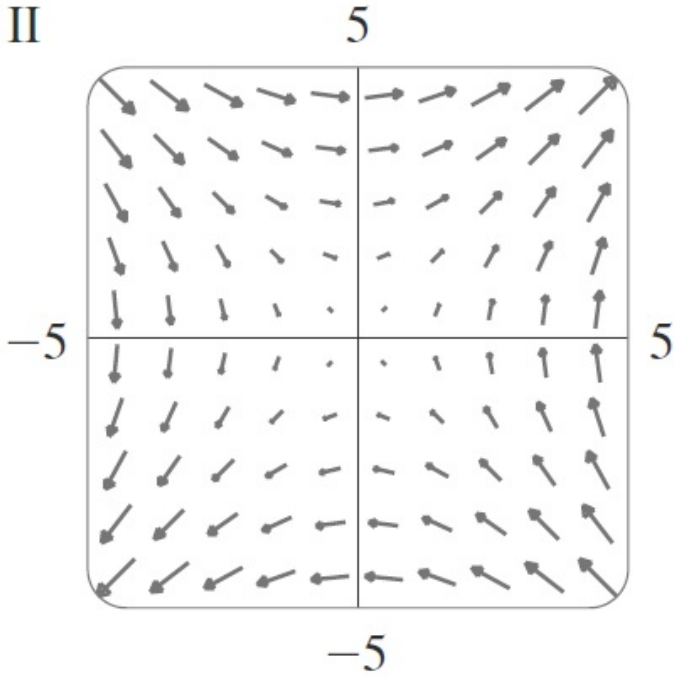
\includegraphics[width=2in]{./img/ej1_II.png}
      \end{figure}
    \end{minipage}
    
  \item $\vecb{F}(x,y)=\pvec{1,\sin{y}}$

    \begin{minipage}{0.5\textwidth}
      Todos los vectores en todos los cuadrantes tienen componentes en $x$ positivas, por lo que apuntan a la derecha todo el tiempo.
      Además cuando $y=\frac{\pi}{2}k$ con $k \in \mathbb{N}$, los vectores estarán alineados horizontalmente. Mientras que si $0 \leq y \leq \pi/2$, los vectores apuntan hacia arriba 
      y si $\pi/2 \leq y \leq \pi$, los vectores apuntan hacia abajo; esto se debe a la función $\sin{}$, la cual modifica la componente vertical del vector. \\
    \end{minipage}%
    \begin{minipage}{0.5\textwidth}
      \begin{figure}[H]
        \centering
        \centering
        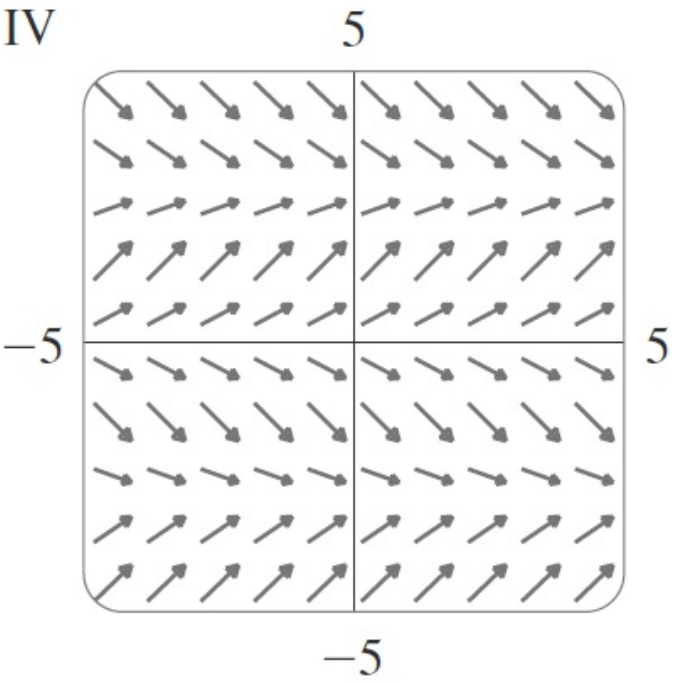
\includegraphics[width=5cm]{./img/ej1_IV.png}
      \end{figure}
    \end{minipage}

    
  \item $\vecb{F}(x,y)=\pvec{x-2,x+1}$

    \begin{minipage}{0.5\textwidth}
      La componente en $x$, $x-2$ indica que los vectores apuntan hacia la izquierda cuando $x<2$ y hacia la derecha cuando $x>2$, manteniendose sin variación en $x=2$.

      La componente en $y$, $x+1$ es positiva para $x>-1$, haciendo que los vectores apunten hacia arriba en esa región, y negativa cuando $x<-1$, haciendo que apunten hacia abajo. En $x=-1$, los vectores estarán alineados horizontalmente.\\
    \end{minipage}%
    \begin{minipage}{0.5\textwidth}
      \begin{figure}[H]
        \centering
        \centering
        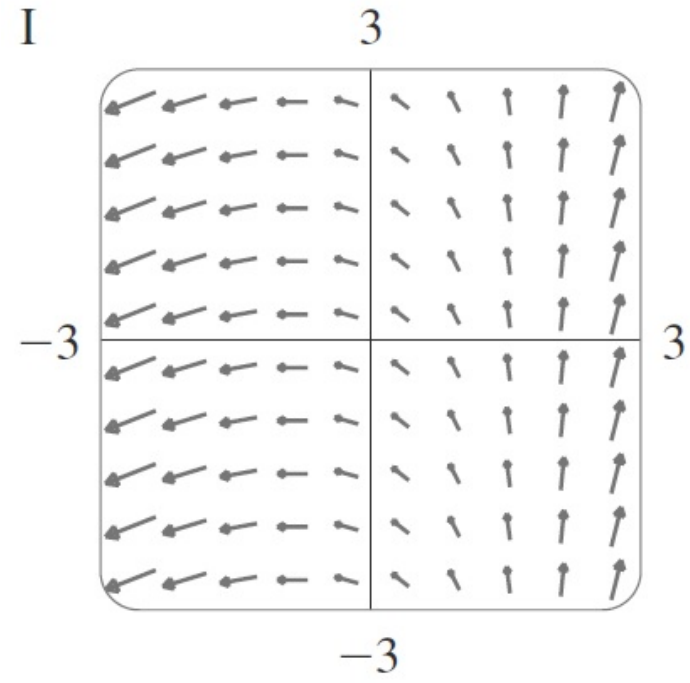
\includegraphics[width=2in]{./img/ej1_I.png}
      \end{figure}
    \end{minipage}

    
  \item $\vecb{F}(x,y)=\pvec{y,1/x}$

    \begin{minipage}{0.5\textwidth}
      Tenemos que cuando $y>0$ (cuadrantes I y II) los vectores tienen componentes en $x$ positivas, apuntan a la derecha, mientas que cuando $y<0$ (cuadrantes III y IV) los vectores tienen componentes en $x$ negativas, apuntan a la izquierda. Por otro lado, cuando $x>0$ la componente vertical es positiva, apuntan hacia arriba, mientras que si $x<0$ la componente vertical es negativa, apuntan hacia abajo.
      Además, La componente en $y=1/x$, es grande cerca del eje $x=0$, disminuyendo a medida que $x$ se aleja de 0.\\
    \end{minipage}%
    \begin{minipage}{0.5\textwidth}
      \begin{figure}[H]
        \centering
        \centering
        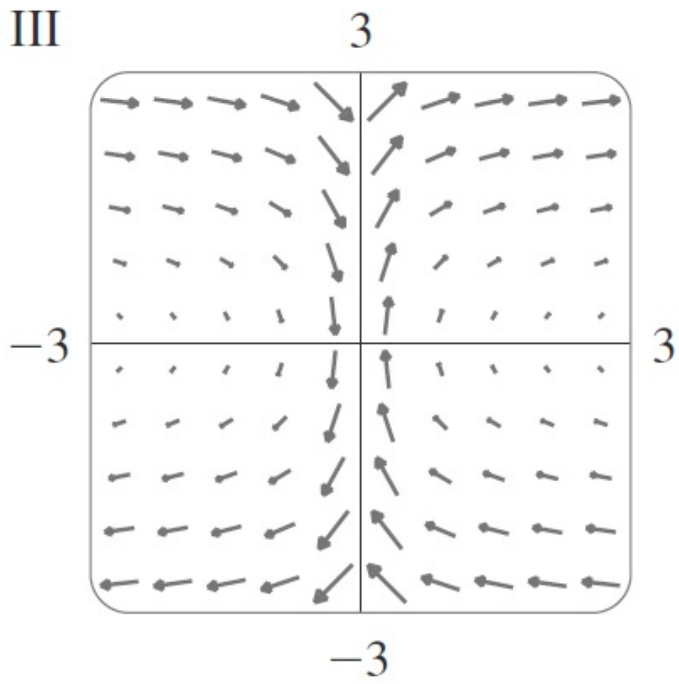
\includegraphics[width=2in]{./img/ej1_III.png}
      \end{figure}
    \end{minipage}
  \end{enumerate}

  % 2
  \question{Relaciona el campo vectorial $\vecb{F}$ con su correspondiente gráfica y da las razones de tu elección:}

  \begin{enumerate}[a)]
  \item $\vecb{F}(x,y,z)=\iuni + 2 \juni + 3 \kuni$

    \begin{minipage}{0.5\textwidth}
      Dado que cada vector tiene componentes constantes en las tres direcciones del espacio: 1 en $x$, 2 en $y$ y $3$ en $z$ (hacia arriba), lo que significa que todos los vectores en cualquier punto tienen la misma dirección y magnitud.
    \end{minipage}%
    \begin{minipage}{0.5\textwidth}
      \begin{figure}[H]
        \centering
        \centering
        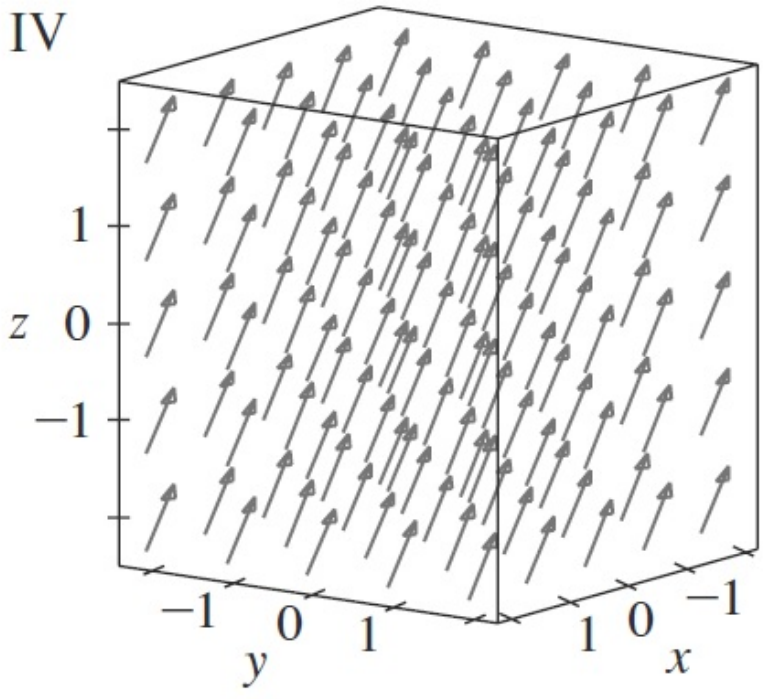
\includegraphics[width=2in]{./img/ej2_IV.png}
      \end{figure}
    \end{minipage}
    
  \item $\vecb{F}(x,y,z)=\iuni + 2 \juni + z \kuni$

    \begin{minipage}{0.5\textwidth}
      Tenemos que cada vector tiene componentes constantes: 1 en $x$ y 2 en $y$. Luego cuando $z>0$ los vectores apuntan hacia arriba, mientras que cuando $z<0$ apuntan hacia abajo, de modo que en $z=0$ permanecen horizontales. 
    \end{minipage}%
    \begin{minipage}{0.5\textwidth}
      \begin{figure}[H]
        \centering
        \centering
        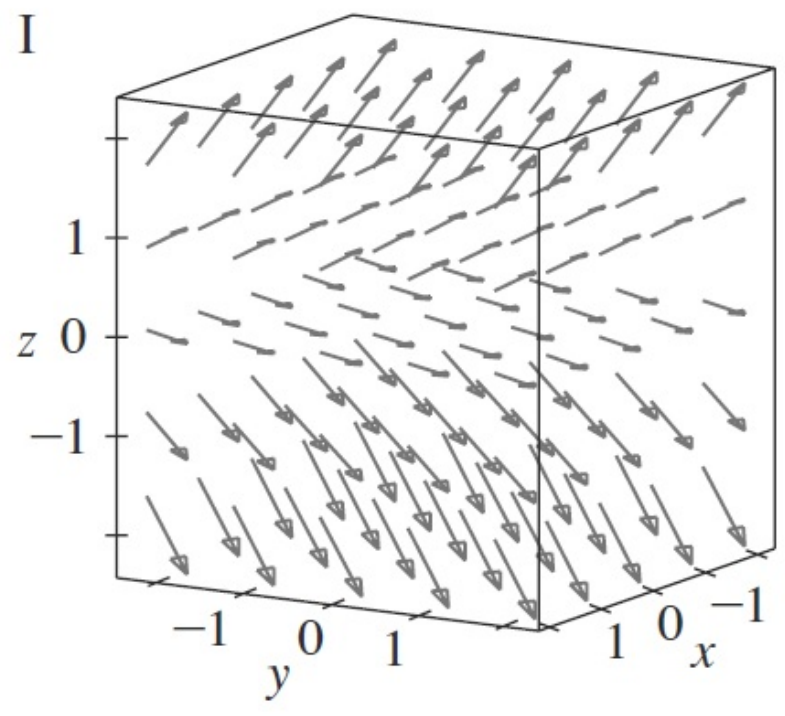
\includegraphics[width=2in]{./img/ej2_I.png}
      \end{figure}
    \end{minipage}
    
  \item $\vecb{F}(x,y,z)=x \iuni + y \juni + 3 \kuni$

    \begin{minipage}{0.5\textwidth}
      Dado que la componente en $z$ es constante, los vectores siempre van a apuntar hacia arriba. Además, los vectores apuntan hacia la derecha cuando \(x > 0\) y hacia la izquierda cuando \(x < 0\), aumentando su magnitud conforme te alejas del origen en la dirección \(x\). De manera similar, la componente en \(y\) es \(y\), por lo que los vectores apuntan hacia arriba cuando \(y > 0\) y hacia abajo cuando \(y < 0\), con una magnitud creciente a medida que aumenta \(y\). 
    \end{minipage}%
    \begin{minipage}{0.5\textwidth}
      \begin{figure}[H]
        \centering
        \centering
        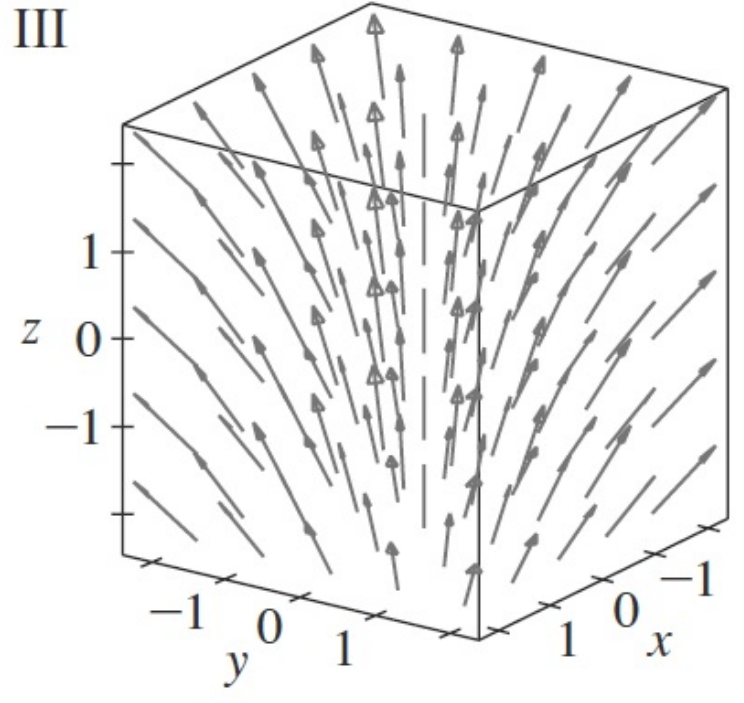
\includegraphics[width=2in]{./img/ej2_III.png}
      \end{figure}
    \end{minipage}

    
  \item $\vecb{F}(x,y,z)=x \iuni + y \juni + z \kuni$

    \begin{minipage}{0.5\textwidth}
      Para cada componente del vector se tiene que si es mayor a cero apuntan hacia arriba y si es menor a cero apuntan hacia abajo, aumentando su magnitud conforme se alejan del origen.
    \end{minipage}%
    \begin{minipage}{0.5\textwidth}
      \begin{figure}[H]
        \centering
        \centering
        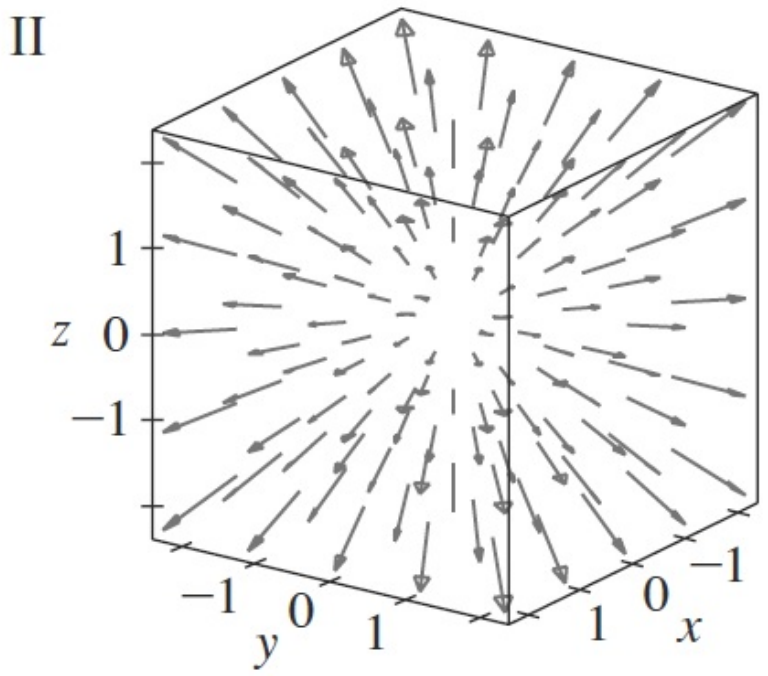
\includegraphics[width=2in]{./img/ej2_II.png}
      \end{figure}
    \end{minipage}
    
  \end{enumerate}

  %3
  \question{Encuentra el campo vectorial gradiente $\nabla f$}
  \begin{enumerate}[a)]
  \item $f(x, y) = \ln{(x + 2y)}$
    \begin{align*}
      \nabla f
      &= \pvec{\frac{\partial f}{\partial x}, \frac{\partial f}{\partial y}} \\
      &= \pvec{\frac{1}{x+2y}\cdot \frac{\partial}{\partial x}( x +2y), \frac{1}{x+2y} \cdot\frac{\partial}{\partial y}( x +2y)} \\
      &= \pvec{\frac{1}{x+2y} \cdot 1, \frac{1}{x+2y} \cdot 2} \\
      &= \pvec{\frac{1}{x+2y}, \frac{2}{x+2y}} \\
    \end{align*}

    $\therefore \nabla f = \pvec{\frac{1}{x+2y}, \frac{2}{x+2y}}$
  \item $f(x, y, z) = \sqrt{x^2+y^2+z^2}$
    \begin{align*}
      &\nabla f\\
      &= \pvec{\frac{\partial f}{\partial x}, \frac{\partial f}{\partial y}} \\
      &= \Big\langle \frac{1}{2\sqrt{x^2+y^2+z^2}}\cdot \frac{\partial}{\partial x}(x^2+y^2+z^2),\\
      &\quad \frac{1}{2\sqrt{x^2+y^2+z^2}}\cdot \frac{\partial}{\partial y}(x^2+y^2+z^2),\\
      & \quad \frac{1}{2\sqrt{x^2+y^2+z^2}}\cdot \frac{\partial}{\partial z}(x^2+y^2+z^2) \Big\rangle \\
      &= \pvec{\frac{1}{2\sqrt{x^2+y^2+z^2}}\cdot 2x,\frac{1}{2\sqrt{x^2+y^2+z^2}}\cdot 2y,\frac{1}{2\sqrt{x^2+y^2+z^2}}\cdot 2z}\\
      &= \pvec{\frac{x}{\sqrt{x^2+y^2+z^2}},\frac{y}{\sqrt{x^2+y^2+z^2}},\frac{z}{\sqrt{x^2+y^2+z^2}}}\\
    \end{align*}

    $\therefore \nabla f = \pvec{\frac{x}{\sqrt{x^2+y^2+z^2}},\frac{y}{\sqrt{x^2+y^2+z^2}},\frac{z}{\sqrt{x^2+y^2+z^2}}}$
  \item $f(x, y) = xy - 2x$
    \begin{align*}
      \nabla f
      &= \pvec{\frac{\partial f}{\partial x}, \frac{\partial f}{\partial y}} \\
      &= \pvec{y-2, x}
    \end{align*}

    $\therefore \nabla f = \pvec{y-2, x}$
  \end{enumerate}

  %4
  \question{Sea $\vecb{F}$ el campo vectorial que se muestra en la siguiente figura}
  \begin{figure}[H]
    \centering
    \centering
    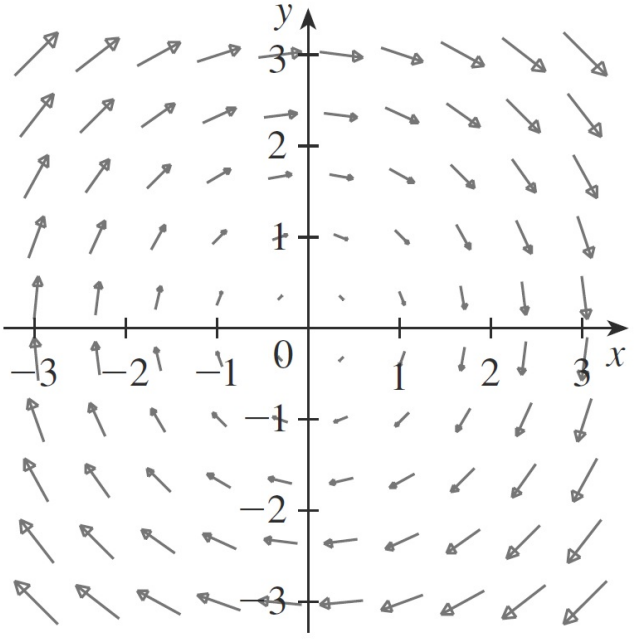
\includegraphics[width=3in]{./img/ej4.png}
  \end{figure}

  \begin{enumerate}[a)]
  \item Si $C_1$ es un segmento de recta vertical que va de (-3, -3) a (-3, 3), determina si
    $\int_{C_1} \vecb{F}\cdot d\vecb{r}$ es \textit{positiva}, \textit{negativa} o \textit{cero}.

    
    $\int_{C_1} \vecb{F}\cdot d\vecb{r}$ es \textit{\textbf{positiva}} puesto que el segmento de recta vertical va de abajo hacia arriba y sobre esa misma linea los vectores del campo tienen componentes $y$ positivas, es decir, van en la misma dirección hacia arriba.

  \item Si $C_2$ es un círculo con orientación antihoraria de radio 3 y con centro en el origen, determina si     $\int_{C_2} \vecb{F}\cdot d\vecb{r}$ es \textit{positiva}, \textit{negativa} o \textit{cero}.

    $\int_{C_2} \vecb{F}\cdot d\vecb{r}$ es \textit{\textbf{negativa}} porque el campo vectorial obstruye el movimiento de la trayectoria a lo largo del círculo con radio 3; esto se debe a que todos los vectores del campo apuntan en el sentido de las manecillas del reloj, mientras que la orientación del círculo es antihoraria.


  \end{enumerate}

  
  
  % 5
  \question{Evalúa la integral de línea $\int_C \vecb{F} \cdot d\vecb{r}$ , donde $C$ esta dada por la función vectorial $\vecb{r}(t)$}

  \begin{enumerate}[a)]
    
  \item $\vecb{F}(x,y) = x^2y^3\iuni - y \sqrt{x} \juni$, con $\vecb{r}(t)=t^2\iuni-t^3\juni, ~ 0\leq t\leq 1$
    \begin{align*}
      \int_C \vecb{F} \cdot d\vecb{r}
      &= \int_0^1 \vecb{F}(\vecb{r}(t)) \cdot \vecb{r}~'(t) ~dt\\
      &= \int_0^1 \vecb{F}(t^2, -t^3) \cdot \pvec{2t, -3t^2} ~dt\\
      &= \int_0^1 \pvec{(t^2)^2(-t^3)^3, -(-t^3)\sqrt{t^2}}  \cdot \pvec{2t, -3t^2} ~dt\\
      &= \int_0^1 \pvec{-t^{13}, t^4}  \cdot \pvec{2t, -3t^2} ~dt\\
      &= \int_0^1 (-t^{13}\cdot 2t) + (-t^4\cdot -3t^2) ~dt\\
      &= \int_0^1 (-2t^{14}) + (-3t^6) ~dt\\
      &= -2 \int_0^1 t^{14} ~dt - 3 \int_0^1 t^6 ~dt\\
      &= -2 \left[ \frac{t^{15}}{15} \right]_0^1 - 3 \left[ \frac{t^7}{7} \right]_0^1\\
      &= -2 \left[ \frac{1}{15} - \frac{0}{15} \right] - 3 \left[ \frac{1}{7} - \frac{0}{7} \right]\\
      &= -2\frac{1}{15} - 3\frac{1}{7}\\
      &= -\frac{59}{105} \\
      &\approx -0.5619
    \end{align*}

    $\therefore \int_C \vecb{F} \cdot d\vecb{r} = -\frac{59}{105} \approx -0.5619$

  \item $\vecb{F}(x,y,z) = \sin{x} \iuni + \cos{y} \juni + xz \kuni$
    con $\vecb{r}(t)=t^3\iuni-t^2\juni+t\kuni, ~ 0\leq t\leq 1$
    \begin{align*}
      \int_C \vecb{F} \cdot d\vecb{r}
      &= \int_0^1 \vecb{F}(\vecb{r}(t)) \cdot \vecb{r}~'(t) ~dt\\
      &= \int_0^1 \vecb{F}(t^3, -t^2, t) \cdot \pvec{3t^2, -2t, 1} ~dt\\
      &= \int_0^1 \pvec{\sin{(t^3)}, \cos{(-t^2)}, t^4}\cdot \pvec{3t^2, -2t, 1} ~dt\\
      &= \int_0^1 3t^2\sin{(t^3)} -2t\cos{(-t^2)} + t^4 ~dt\\
      &= \left[ -\cos{t^3} + \sin{(-t^2)} + \frac{t^5}{5} \right]_{t=0}^{t=1}\\
      &= \left[ -\cos{t^3} - \sin{t^2} + \frac{t^5}{5} \right]_{t=0}^{t=1}\\
      &= \left[ -\cos{1} - \sin{1} + \frac{1}{5}\right] - \left[ -\cos{0} - \sin{0} + \frac{0}{5} \right]\\
      &= \left[ -\cos{1} - \sin{1} + \frac{1}{5}\right]-\left[-1-0+0\right]\\
      &= \frac{6}{5} -\cos{1} - \sin{1}
    \end{align*}

    $\therefore \int_C \vecb{F} \cdot d\vecb{r} =\frac{6}{5} -\cos{1} - \sin{1}$

  \item $\vecb{F}(x,y) = e^{x-1}\iuni + xy \juni$, con $\vecb{r}(t)=t^2\iuni +t^3 \juni, ~ 0\leq t\leq 1$
    \begin{align*}
      \int_C \vecb{F} \cdot d\vecb{r}
      &= \int_0^1 \vecb{F}(\vecb{r}(t)) \cdot \vecb{r}~'(t) ~dt\\
      &= \int_0^1 \vecb{F}(t^2,t^3) \cdot \pvec{2t,3t^2} ~dt\\
      &=  \int_0^1 \pvec{e^{t^2-1},t^5} \cdot \pvec{2t,3t^2} ~dt\\
      &= \int_0^1 2te^{t^2-1} + 3t^7 ~dt\\
      &= \left[e^{t^2-1}+\frac{3t^8}{8}\right]_0^1\\
      &= (e^0+3/8)-(e^{-1})\\
      &= \frac{11}{8} - \frac{1}{e}
    \end{align*}

    $\therefore \int_C \vecb{F} \cdot d\vecb{r} =\frac{11}{8} - \frac{1}{e}$
  \end{enumerate}

  % 6
  \question{Encuentra el trabajo realizado por el campo de fuerza 
    $\vecb{F}(x, y) = x\iuni + (y + 2)\juni$ al mover unobjeto a lo largo del cicloide 
    $\vecb{r}(t) = (t-\sin{t})\iuni + (1-\cos{t})\juni$ con $0\leq t\leq 2\pi$.}
  \begin{align*}
    W
    &= \int_0^{2\pi} \vecb{F}(\vecb{r}(t)) \cdot \vecb{r}~'(t) ~dt\\
    &= \int_0^{2\pi} \pvec{t-\sin{t}, (1-\cos{t})+2} \cdot \pvec{1-\cos{t}, \sin{t}} ~dt\\
    &= \int_0^{2\pi} \pvec{t-\sin{t}, 3-\cos{t}} \cdot \pvec{1-\cos{t}, \sin{t}} ~dt\\
    &= \int_0^{2\pi} (t-\sin{t})(1-\cos{t}) + \sin{t}(3-\cos{t}) ~dt \\
    &= \int_0^{2\pi} (t-\sin{t}-t\cos{t}+\sin{t}\cos{t}) + (3\sin{t}- \sin{t}\cos{t}) ~dt\\
    &= \int_0^{2\pi} (t -t\cos{t} + 2\sin{t}) ~dt\\
    &= \int_0^{2\pi} (t + 2\sin{t}) ~dt - \int_0^{2\pi} t\cos{t}~dt \\
    &= \left[\frac{t^2}{2}-2\cos{t}\right]_{t=0}^{t=2\pi} - \int_0^{2\pi} t\cos{t}~dt \\
    &=      \left[\left(\frac{4\pi^2}{2}-2\cos{(2\pi)}\right)-\left(\frac{0}{2}-2\cos{0}\right)\right]- \int_0^{2\pi} t\cos{t}~dt \\
    &= (2\pi^2 - 2 + 2)- \int_0^{2\pi} t\cos{t}~dt \\
    &= 2\pi^2- \int_0^{2\pi} t\cos{t}~dt 
  \end{align*}

  Integrando por partes: Sea $u=t$, $dv=\cos{t}~dt$, entonces $du=dt$ y $v=\sin{t}$. Así
  \begin{align*}
    \int_0^{2\pi} t\cos{t}~dt
    &= t\sin{t}\Big|_0^{2\pi} - \int_0^{2\pi} \sin{t}~dt \\
    &= (2\pi\sin{(2\pi)}-0\sin{0})-\left[-\cos{t}\right]_0^{2\pi}\\
    &= (0-0) + (\cos{2\pi}-\cos{0})\\
    &= 1-1\\
    &=0
  \end{align*}

  Sustitutendo en $2\pi^2- \int_0^{2\pi} t\cos{t}~dt $, tenemos que $W= 2\pi^2$

  $\therefore W= 2\pi^2$

  % 7
  \question{}
  \begin{enumerate}[a)]
  \item Muestra que un campo de fuerzas constante ($\vecb{F} = \pvec{a,b}$) no realiza trabajo sobre una
    partícula que se mueve uniformemente una vez alrededor del círculo $x^2+y^2=1$.

    Primero, veamos que el círculo unitario puede parametrizarse por $\vecb{r}(t) = \cos{t} \iuni + \sin{t} \juni$ con $0\leq t\leq 2\pi$.
    Entonces, el trabajo esta dado por
    \begin{align*}
      W
      &= \int_0^{2\pi} \vecb{F}(\vecb{r}(t)) \cdot \vecb{r}~'(t) ~dt\\
      &= \int_0^{2\pi} \pvec{a, b} \cdot \pvec{\cos{t}, \sin{t}} ~dt\\
      &= \int_0^{2\pi} a\cos{t} + b\sin{t} ~dt\\
      &= \left[a\sin{t} -b\cos{t} \right]_0^{2\pi}\\
      &= (a\sin{2\pi} -b\cos{2\pi}) - (a\sin{0} -b\cos{0})\\
      &= (0-b)-(0-b)\\
      &= 0
    \end{align*}

    $\therefore W= 0$. Esto demuestra que un campo de fuerzas constante no realiza trabajo sobre una partícula que se mueve uniformemente una vez alrededor del círculo $x^2+y^2=1$.

  \item ¿Lo anterior también es cierto para el campo de fuerzas $\vecb{F}(\vecb{x}) = k\vecb{x}$, donde $k$ es una constante y $\vecb{x}=\pvec{x,y}$?

    Tenemos que el trabajo está dado por
    \begin{align*}
      W
      &= \int_0^{2\pi} \vecb{F}(\vecb{r}(t)) \cdot \vecb{r}~'(t) ~dt\\
      &= \int_0^{2\pi} k\pvec{x,y} \cdot \pvec{\cos{t}, \sin{t}} ~dt\\
      &= \int_0^{2\pi} kx\cos{t} + ky\sin{t} ~dt\\
      &= \left[kx\sin{t} - ky\cos{t} \right]_0^{2\pi}\\
      &= (kx\sin{2\pi} - ky\cos{2\pi}) - (kx\sin{0} - ky\cos{0})\\
      &= (0-ky)-(0-ky)\\
      &= 0
    \end{align*}

    $\therefore W= 0$. Esto demuestra que un campo de fuerzas $\vecb{F}(\vecb{x}) = k\vecb{x}$, donde $k$ es una constante y $\vecb{x}=\pvec{x,y}$ no realiza trabajo sobre una
    partícula que se mueve uniformemente una vez alrededor del círculo $x^2+y^2=1$

  \end{enumerate}


\end{questions}

























\vskip30pt
\RaggedRight

\newpage


\newgeometry {
  hmargin = {1.5cm, 1.5cm},
  vmargin = {5cm, 1cm},
  nohead,			% Elimina el encabezado
  nomarginpar,	% Elimina las notas
  includeall,
}% \savegeometry{geometria_1}

\pagestyle{foot}    % El estilo de ésta página sólo constará de pié de página
\runningfooter{}{}{Página \thepage\ de \numpages}

\end{document}
